\documentclass{ximera}
\input{../preamble}
\addPrintStyle{..}
\begin{document}
	\author{Zomercursus KU Leuven}
	\xmtitle{Het complexe vlak}{Een meetkundige voorstelling van de complexe getallen}
	\label{xim:cmplx_definitie_complexe_vlak}

Een complex getal $z=a+bi\in \C$ kan worden beschouwd als een punt in het reële  vlak, namelijk als het punt
met cartesiaanse coördinaten $(a,b)$ (met $a,b$ dus reële getallen). 

\begin{image}[0.3\textwidth]
	\begin{tikzpicture}[scale=3]%,cap=round,transform canvas={scale=0.5}]
	
	\tikzmath{\hoek = 35; \myc = cos(\hoek); \mys = sin(\hoek); 
		\hoekb = 20;}
	
		% Goniometrische cirkel
%	\draw (0,0) circle (1cm);
	\draw[->] (-0.1,0) -- (1.2,0) node[above] {$\Re(z)$};
	\draw[->] (0,-0.1) -- (0,1) node[right] {$\Im(z)$};

	\draw[color=blue,thick] (0:0)  -- (\hoek:1); 
	%
	\draw[color=black] (\hoek:1) node[name=P,circle, fill=black, radius=1pt,scale=0.8] {} node [yshift=2pt,above] {$z=a+bi$} ;  
	%
	\draw[dashed] ({cos(\hoek)},0) node[circle, fill=black, radius=1pt,scale=0.5] {} node[below] {$a$} -- (P);
	\draw[dashed] (0,{sin(\hoek)}) node[circle, fill=black, radius=1pt,scale=0.5] {} node[left] {$b$} -- (P);
	%
	\draw [thick, red,decorate,decoration={brace,amplitude=10pt,mirror},yshift=-5pt](0,0) -- ({cos(\hoek)},0) node[black,midway,yshift=-0.6cm] {\footnotesize $a$};
	%
	\draw [thick, red,decorate,decoration={brace,amplitude=10pt},xshift=-5pt](0,0) -- (0,{sin(\hoek)}) node[black,midway,left,xshift=-8pt] {\footnotesize $b$};
	
	\end{tikzpicture}

\end{image}

De schrijfwijze $a+bi$ van een complex getal noemt men de \textbf{cartesiaanse vorm}.
We spreken in deze context ook van \textbf{het complexe vlak} of \textbf{het vlak van Gauss}.
\\
De \textbf{zuiver reële} getallen bevinden zich op de (horizontale) $x-$as, die we dan ook de \textbf{reële as} noemen.
\\
De \textbf{zuiver imaginaire} getallen bevinden zich op de (verticale) $y-$as, die we de \textbf{imaginaire as} noemen.

Door deze voorstelling van een complex getal in een vlak kan je ook meetkundig redeneren bij de bewerkingen met complexe getallen. Zo komt de optelling overeen met de optelling van vectoren volgens de regel van het parallellogram. Vermenigvuldigen met $i$ is hetzelfde als een rotatie met $90$ graden. Daaruit volgt dat het kwadraat van $i$ overeenkomt met een rotatie van $180$ graden, en dat is precies hetzelfde als vermenigvuldigen met $-1$. In die zin is $i$ dus wel degelijk een vierkantswortel uit $-1$. Het blijkt dadelijk dat ook $-i$ een vierkantswortel is van $i$.

\begin{image}[\textwidth]
	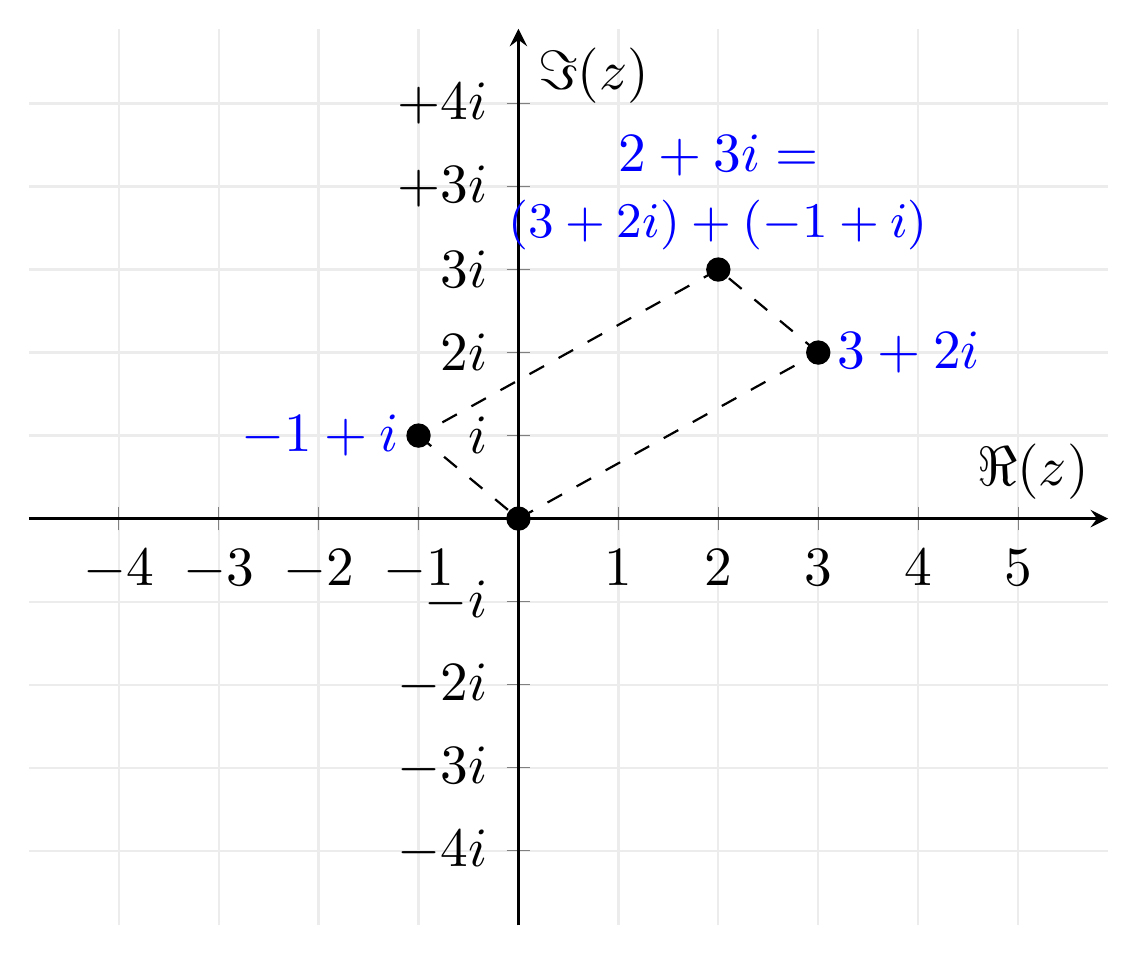
\begin{tikzpicture}[scale=2]
	\begin{axis}
	[
	ytick ={-7,...,8}, yticklabels={$-7i$, $-6i$, $-5i$, $-4i$, $-3i$, $-2i$, $-i$, $0$, $i$, $2i$, $3i$, $+3i$, $+4i$, $+5i$, $+6i$, $+7i$, $+8i$},
	xtick ={-7,...,8},
	axis lines = center, 
	enlargelimits,
	grid=both,
	grid style={gray!15},
	% minor tick num=1,
	ticks=both,
	xlabel=$\Re(z)$,
	ylabel=$\Im(z)$,
	ymin=-4,
	ymax=+5,
	xmin=-4,
	xmax=+5
	]
	
	\addplot [black, mark = *] coordinates {( 0, 0)} {};
	\addplot [black, mark = *] coordinates {( 3, 2)} {};
	\addplot [black, mark = *] coordinates {( 2, 3)} {};
	\addplot [black, mark = *] coordinates {( -1, 1)} {};
	
	\node [below right, blue] at (axis cs:  0, 0) {};
	\node [right, blue] at (axis cs:  3, 2) {$3+2i$};
	\node [above, blue,align=center] at (axis cs:  2, 3) {$2+3i = $\\ \small$(3+2i) + (-1+i)$};
	\node [left, blue] at (axis cs:  -1, 1) {$-1+i$};
	
	\addplot [dashed, black] coordinates { (0,0) (3,2) };
	\addplot [dashed, black] coordinates { (3,2) (2,3) };
	\addplot [dashed, black] coordinates { (2,3) (-1,1) };
	\addplot [dashed, black] coordinates { (-1,1) (0,0) };
	
	\end{axis}
	\end{tikzpicture}
	\qquad
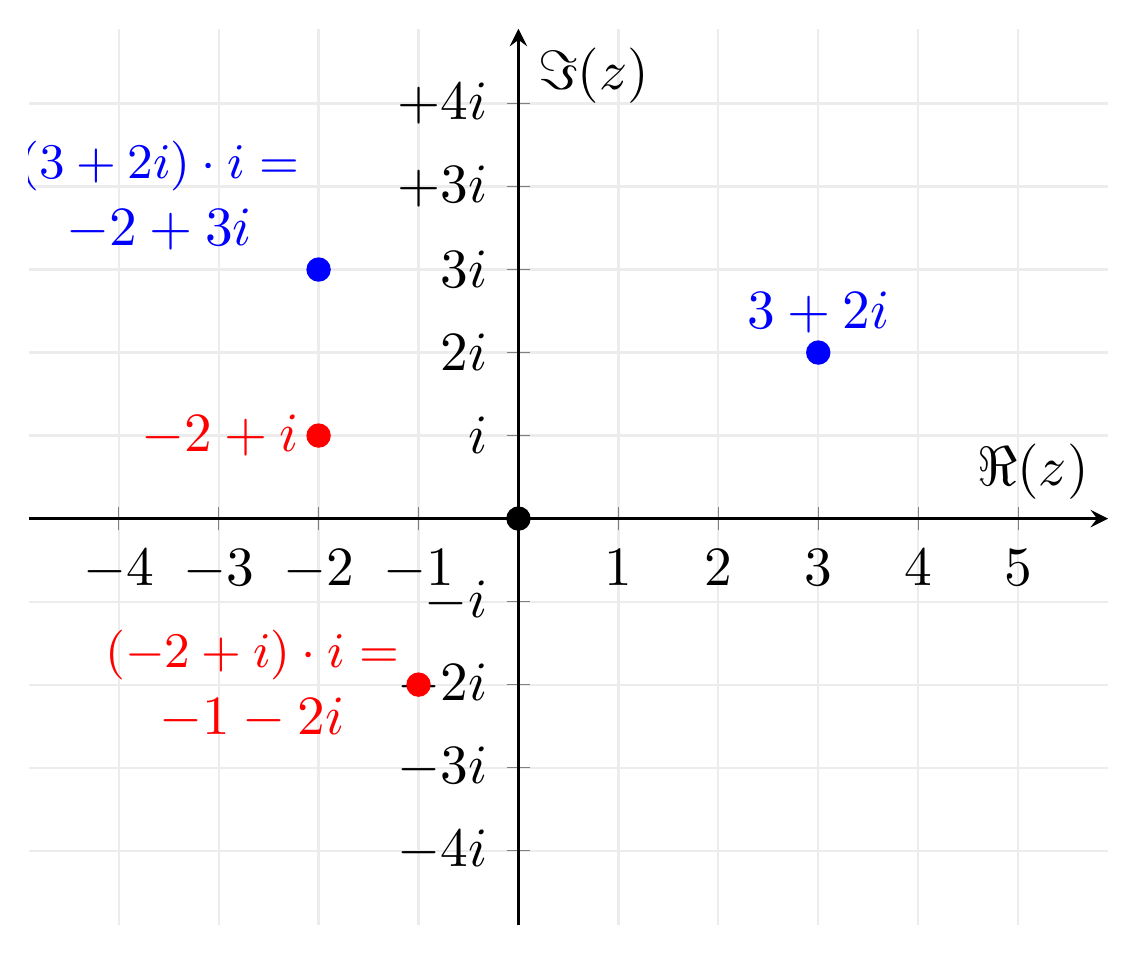
\begin{tikzpicture}[scale=2]
	% TODO: rotatie van 90 graden beter aanduiden !
\begin{axis}
[
	ytick ={-7,...,8}, yticklabels={$-7i$, $-6i$, $-5i$, $-4i$, $-3i$, $-2i$, $-i$, $0$, $i$, $2i$, $3i$, $+3i$, $+4i$, $+5i$, $+6i$, $+7i$, $+8i$},
	xtick ={-7,...,8},
	axis lines = center, 
	enlargelimits,
	grid=both,
	grid style={gray!15},
ticks=both,
xlabel=$\Re(z)$,
ylabel=$\Im(z)$,
ymin=-4,
ymax=+5,
xmin=-4,
xmax=+5
]

\addplot [black, mark = *] coordinates {( 0, 0)} {};

\addplot[blue,mark=*] coordinates {(3,2)} node[above] {$3+2i$};
\addplot[blue,mark=*] coordinates {(-2,3)} node[above left, align=center] {\small$(3+2i)\cdot i =$\\$ -2+3i$};

\addplot[red,mark=*] coordinates {(-2,1)} node[left] {$-2+i$} ;
% \addplot[red,mark=*] coordinates {(-2,1)} node[pin=150:{$-2+i$}]{} ;
\addplot[red,mark=*] coordinates {(-1,-2)} node[left,align=center]{\small$(-2+i)\cdot i =$\\$-1-2i$};
% todo: aanduiden rotatie 90degree!
\end{axis}
\end{tikzpicture}
\end{image}

\end{document}
